\chapter{Single \hisparc station}
\label{ch:station}

\section{Signal digitization}

The signal in one channel is sampled by two \adcs. To get good data and triggering the \adcs need to be calibrated to have the same baseline and response (gain). The \adcs normally have a range of \SIrange{-1}{1}{\volt} translated into a 12-bit value. This is good for AC signals, but the \pmt outputs negative pulses. Any positive pulses are less important, but can be used to detect reflections. An electric circuit in the \hisparc electronics modifies the incoming signal to increase the dynamic range for the DC pulses. The baseline of the signals is calibrated to make an input of \SI{0}{\volt} correspond to \SI{200}{\adc} (\hisparcii) or \SI{30}{\adc} (\hisparciii). The gain is such to get a conversion factor of \SI{-0.57}{\milli\volt\per\adc} (\hisparcii) or \SI{-0.584}{\milli\volt\per\adc} (\hisparciii). This results in an effective range of \SIrange{-2.222}{0.113}{\volt} (\hisparcii) or \SIrange{-2.374}{0.018}{\volt} (\hisparciii).

The two thresholds used for the trigger are \SI{-30}{\milli\volt} (low) and  \SI{-70}{\milli\volt} (high). These correspond to \SI{53}{\adc} (\hisparcii) or \SI{50}{\adc} (\hisparciii), and \SI{123}{\adc} (\hisparcii) or \SI{120}{\adc} (\hisparciii) above the baselines. However, for some stations slightly different threshold may be used, the chosen thresholds are sent to the datastore as part of the station configuration. In the data processing the thresholds from the configuration data need to be used for trigger time reconstruction.


\subsection{\adc sampling}

The \pmt signals are sampled every \SI{2.5}{\ns} alternately by the two \adcs.
In order to get consistent data both \adcs are aligned to have the same baseline and gain. \adcs remain accurate when they have a constant temperature. When \hisparc electronics are first connected the temperature will likely be below operating temperature. When calibration is performed immediately after powering the electronics it may drift from proper calibration as it continues to operate [how much drift?]. An offline/software based Mean Filter [ref to later section] in the software is capable of smoothing the combined signal. This removes any small misalignment effects. Slightly different gains can cause very bad alignment at higher voltages. An example of misaligned traces is shown in \cref{fig:adc_alignment}.

\begin{figure}
    \centering
    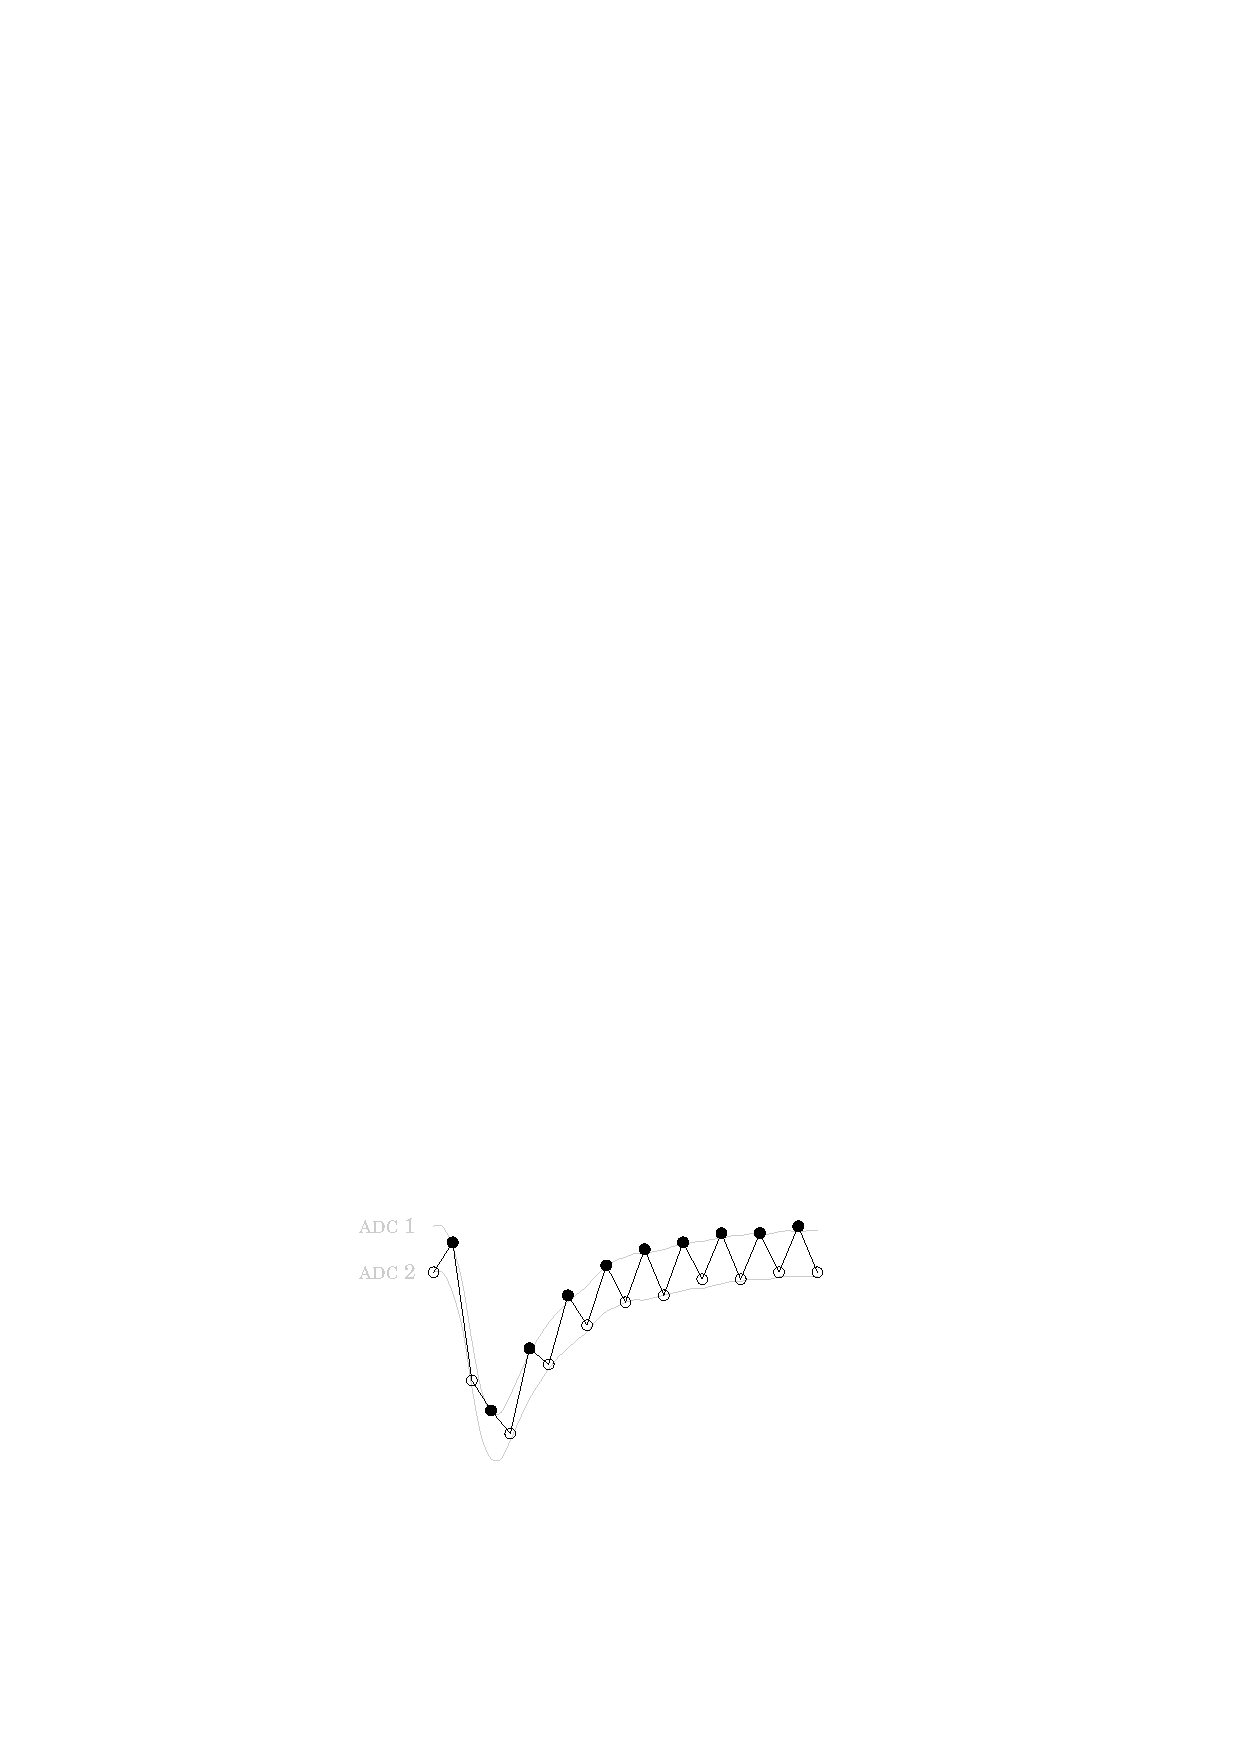
\includegraphics{plots/station/adc_alignment}
    \caption{Signals are read by two \adcs alternatively (open and closed circles). When the \adcs are not properly aligned they return different results for the same input.}
    \label{fig:adc_alignment}
\end{figure}


\subsection{Comparators}

LiO 2011 - Marcelis?

The non-linearity of the \pmt response described in the previous chapter means that many \pmts will never saturate the \adcs. The \hisparc electronics also includes two comparators per channel which determine if a signal reaches two higher thresholds (\SIrange{2}{10}{\volt}). These will remain unused with most stations. For the new \pmts the comparators will be essential in signal reconstruction of high particle densities. However, the readout of the comparators was not implemented in the software until the end of 2015. So these will not be taken into further account in this thesis.


\section{Timing}


\subsection{Trigger time and the Mean Filter}

An additional effect of misalignment is the probability of either \adc being the one which causes a trigger. An \adc with a slightly higher baseline (in \adc counts) is more likely to cause a trigger. This effect is reduced when looking at events with higher particles densities because the rise time of the pulses is reduced. (or steepness of pulse front is higher). This can be seen in [figure with histogram of trigger time], the reconstructed trigger time has a preference for one of the two channels. The preference matches the ADC which has a higher baseline.

In the DAQ software used before 2016 activating the Mean Filter would also apply the filter on the traces being sent to the datastore. This is not desirable because the reconstruction of the trigger time in the event requires unfiltered traces. However, in most cases trigger reconstruction will be successful on filtered traces, unless the pulse heights are very close to the thresholds used in the trigger. In that case the filter may reduce the signal to values below the threshold making reconstruction impossible, since the filter is destructive/irreversible.


\subsection{Mean Filter and trigger reconstruction}

The misalignment of the \adcs also affects the arrival time reconstruction. However, to reduce the preference for either \adc the mean filter can be applied to unfiltered traces before reconstructing arrival times.

- Rise time effect on arrival time reconstruction.


\subsection{Detector offset calibration}

- [figure] arrival time distribution between two detectors in a station
  Detector offsets can be determined with a day of data (accuracy?). Arrival
  time differences give an almost Guassian distribution.


- [figure] timeline of changes in detector offsets in a station

\begin{figure}
    \centering
    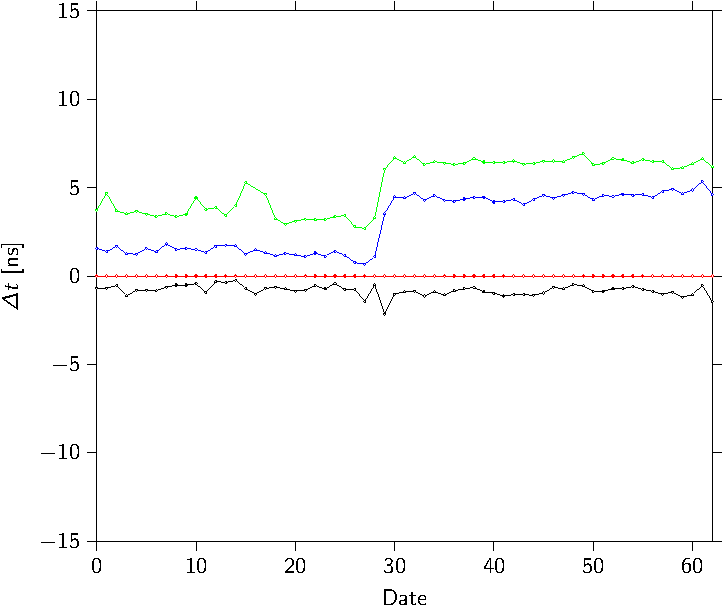
\includegraphics{plots/station/detector_offset_drift_month_501}
    \caption{This shows the changes in detector offsets for the detectors of station 501. Detector two is used as reference. The large jump observed for detector 3 (green) and 4 (blue) was caused by the use of \hisparciii electronics.}
    \label{fig:detector_offset_drift_month_501}
\end{figure}

  Changes in the offsets can be caused by changing the voltages of the PMT, or
  replacing part of the detector, or hisparc electronics. If no changes are
  made the offsets are very stable.
- [figure] distribution of detector offsets between Master detectors


\begin{figure}
    \centering
    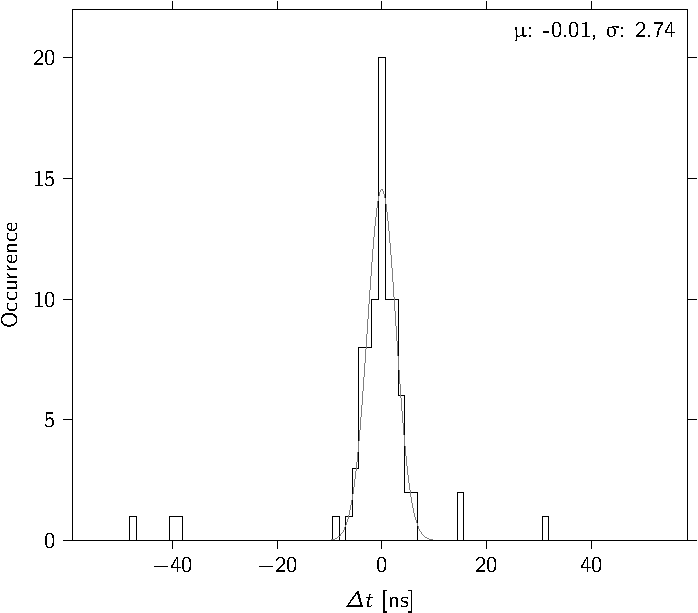
\includegraphics{plots/station/detector_offset_distribution}
    \caption{Distribution of detector offsets. The detector offsets between the two detectors connected to the Master electronics for all \hisparc stations are shown.}
    \label{fig:detector_offset_distribution}
\end{figure}

  Often small offsets, with some outliers. The outliers also remain stable
  over time, so not simply a day of bad data.

- [figure] distribution of detector offsets between master and slave
  [figure] time delta distribution (depends on trigger slave/master?)


\begin{figure}
    \centering
    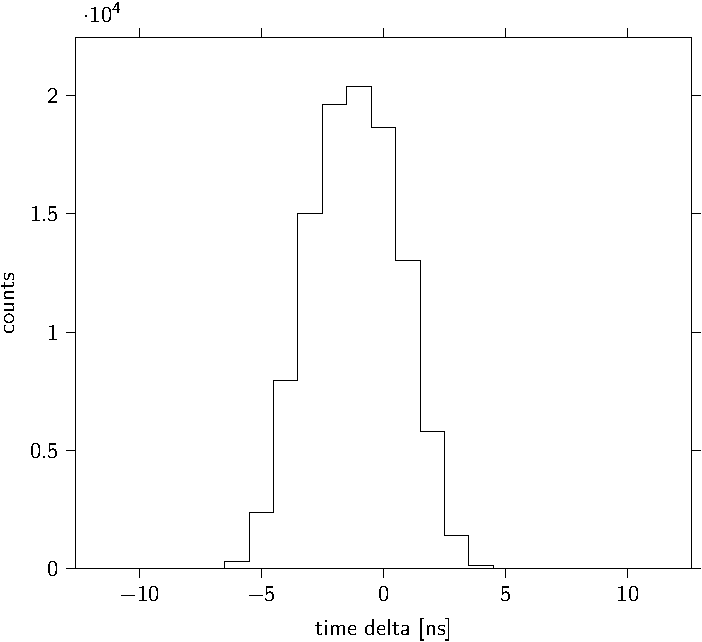
\includegraphics{plots/station/time_delta_501}
    \caption{.}
    \label{fig:time_delta_501}
\end{figure}


The Master and Slave determine their own timestamp for events. The difference between these timestamps is not stored, it is only used to find events that belong together on the station PC. The overal offset between master/slave is corrected for by correcting for detector offsets, small error remains.


\section{Station layouts}

Not all station locations are able to fit the suggested layouts. So slightly modified versions exist. Moreover, not every station is angled the same way relative to North. The detector locations are essential for direction reconstruction, if the angle of a station is not known the reconstructed directions will point to the wrong place on the sky.

\gps positions are automatically submitted by the station to the datastore. Detector positions are not measured automatically, so they need to be measured by hand. Since the \gps antenna position is known, the detector positions relative to the \gps are desired. The coordinate system used to describe detector positions is described in \cref{ch:coordinates}. Moreover, in some stations detectors have been moved into a new configuration, sometimes more than once. Each time the detector positions relative to the then-current position of the \gps need to be determined, including the time of the change. Only if relative position of \gps and detectors change must a new position be submitted. Station supervisors can submit their measured layout, which will be reviewed by one of the \hisparc coordinators. Satellite imagery can sometimes be used to verify the positions of the detectors. These variable detector and \gps positions are taken into account when reconstructing showers.

In \cref{fig:locations_501} the different \gps and detector locations for station 501 are shown. The outlier \gps locations are caused by the usage of temporary \gps antenna during tests. The station layout described by the clustered positions describes the original star-layout, an equilateral triangle with one detector in the center. When station 510 was built station 501 was also moved to create overlapping diamond-shaped stations. Detector 3 (green) was not moved during this transition. For each physical \gps location (including the temporary test locations) the relative detector positions have been measured. Other Science Park stations for which the detectors have been moved are 502 and 505. For station 505 this was done multiple times because alterations to the roof on which the detector reside required them to be moved.

\begin{figure}
    \centering
    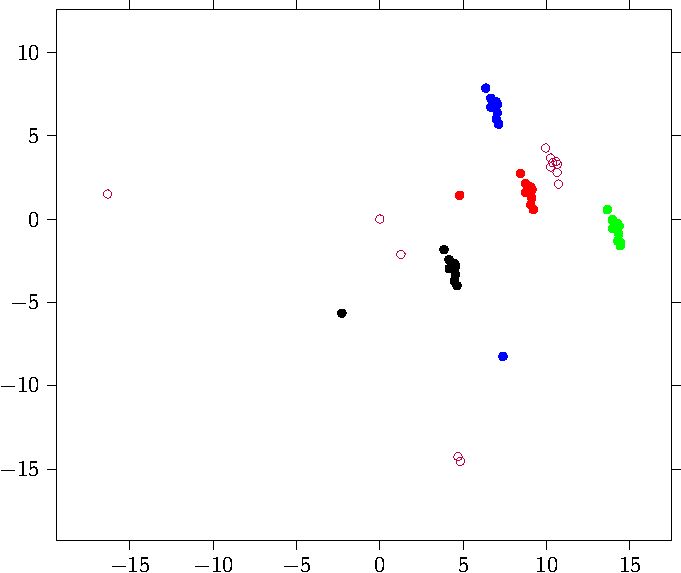
\includegraphics{plots/station/locations_501}
    \caption{Detector (closed circles) and \gps locations (open circles) for station 501. Over time the detectors and \gps antenna for station 501 have been moved multiple times. The large clusters of circles are not necessarily movement of the \gps and detectors but merely new self-surveys by the \gps resulting in a slightly different position.}
    \label{fig:locations_501}
\end{figure}


\section{Overlapping stations}

Station 510 was created to overlap with station 501. Because of the nearly identical detector positions the stations often detect the same showers. Because of this the trigger efficiency and reconstruction accuracy between the two can be compared. These stations work independently, like other stations.


\subsection{Detection efficiency}

The detection efficiency is defined as the probability of a detection given a certain event/particle density. This is determined by checking if the stations are in coincidence or not. For all events in a particle density bin for one station the number of simultaneous events in the other station is counted. These values are then divided to get the probability of an event in the other station given a particle density. In this case we do not know the exact particle density and the station used as reference is also affected by its own detection effciency. So in fact the efficiency of both stations is combined. In \cref{fig:effiency_501_510} the detection(/coincidence?) effiency for 501 (solid) and 510 (dashed) are shown, given a particle density in the other station.

\begin{figure}
    \centering
    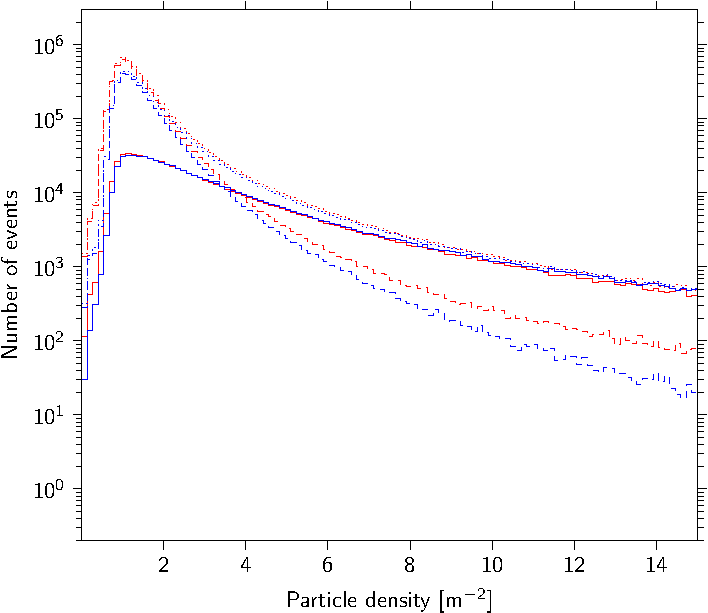
\includegraphics{plots/station/anti_coincidences}
    \caption{Detection efficiency in stations 501 (solid) and 510 (dashed) versus the density measured by the other station. TODO: new plot, currently divide solid by dotted to get effiency.}
    \label{fig:effiency_501_510}
\end{figure}

At a particle density of approximately \SI{3.5}{\per\square\meter} in one station the coincidence probability for the other station becomes \SI{50}{\percent}. At approximately \SI{2.2}{\per\square\meter} the detection probability becomes \SI{25}{\percent} (i.e. \SI{$50^2$}{\percent}).


\subsection{Reconstruction accuracy}

For events in coincidence the direction reconstructions can be compared to see the distance between the reconstructions. For events with higher particle counts the direction reconstruction accuracy increases. This is because of several reasons. First, the probability of detecting a particle from the front of the shower front increases. Secondly, increased probability that a particle hits the detector close to the \pmt, reducing the transport time. Thirdly, the rise time of the signal decreases. Fourthly, the increased particle density increases the probability of being close to the shower core, where the shower front is more flat, which is assumed in the reconstruction.

\begin{figure}
    \centering
    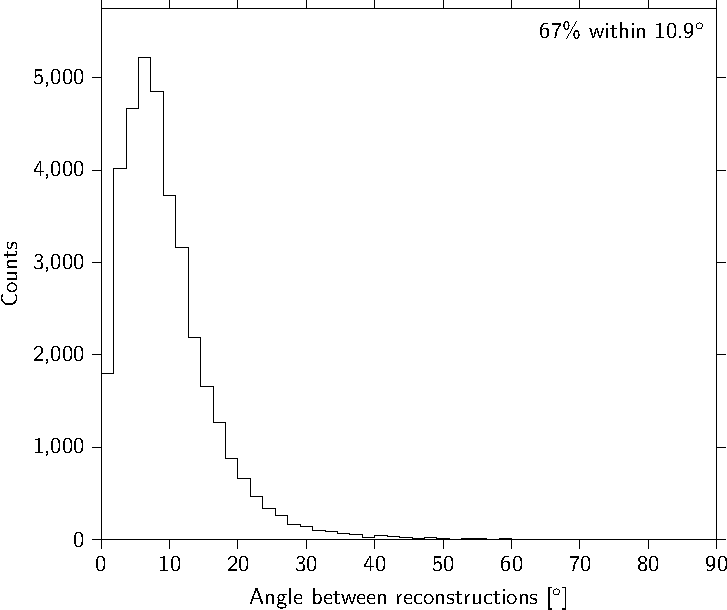
\includegraphics{plots/station/angle_between_501_510_minn2}
    \caption{Angle between the direction reconstruction in coincident events between station 501 and 510.}
    \label{fig:angle_between_501_510}
\end{figure}



- eis beide buitenste detector veel deeltjes. in vergelijking aantal deeltjes in coincidenties
